% portail-publications.tex
\section{Mes publications.}
Dans l'onglet \bsc{publications} sont regroupées toutes les publications que vous avez rédigées, publications forcément associées à un groupe.
\begin{figure}
	\centering
	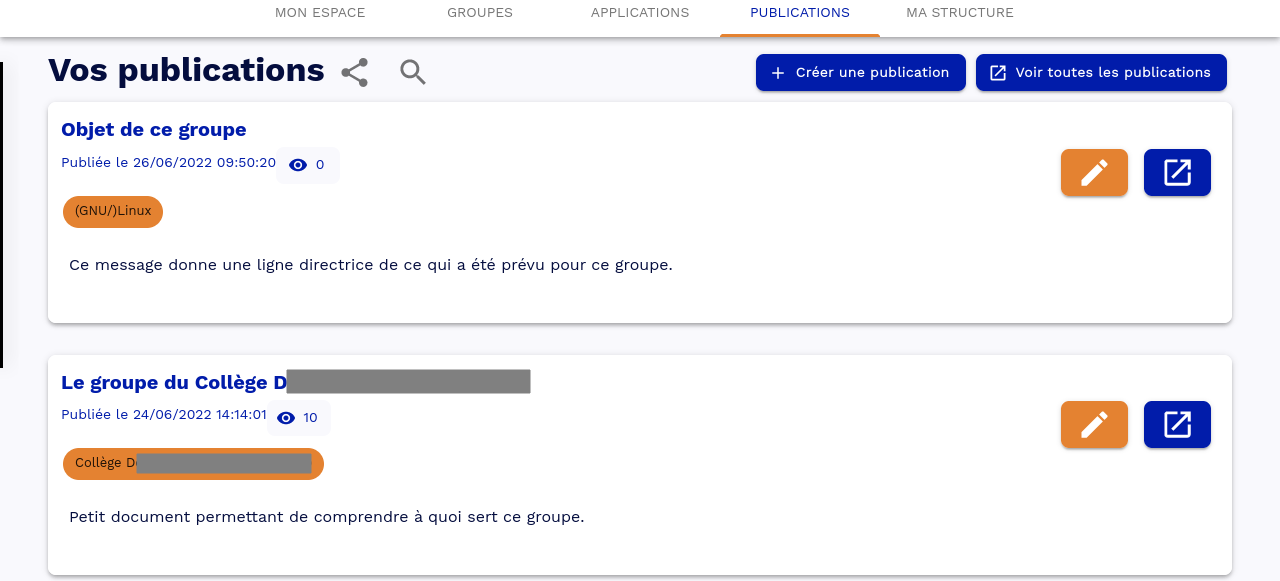
\includegraphics{./Captures/portail.publications.exemples.png}
	\caption{Exemples de publications personnelles.}
\end{figure}
Les seules options importantes sont regroupées vers la droite, il s'agit des gros boutons bleus pour
\begin{itemize}
	\item[+] Créer une publication
	\item[$\square$] Voir toutes les publications
\end{itemize}

Au sein d'une ligne de publication, les deux icônes importantes sont l'icône orange pour modifier une publication déjà rédigée, et pour afficher cette publication

\subsection{Créer une publication}
Lors de l'appui sur le bouton de création, une nouvelle fenêtre s'ouvre et les différents champs apparaissent. 
\begin{figure}
	\centering
	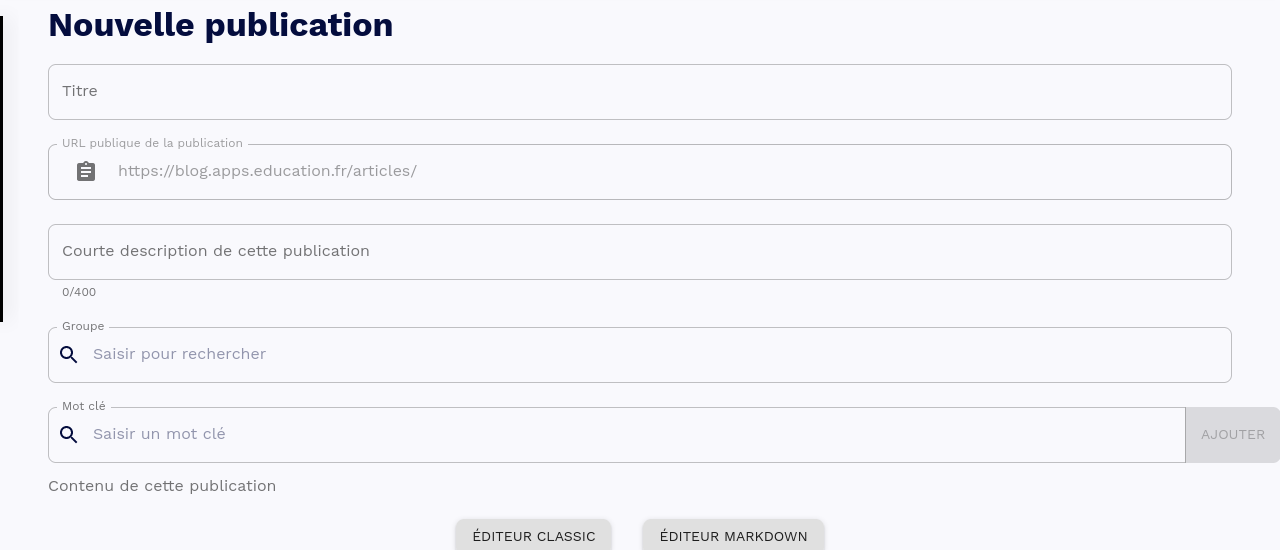
\includegraphics{./Captures/portail.publications.creer.publication.1.png}
	\caption{La première partie lors de la création d'une publication.}
\end{figure}
Parmi eux certains sont forcément obligatoires, en l'occurrence le titre bien sûr mais également le groupe dans lequel cette publication apparaîtra.

La partie inférieure de la fenêtre affiche deux options pour la publication et des boutons correspondants, à savoir l'éditeur classique ou l'éditeur markdown.

\paragraph{L'éditeur classique} affiche une barre d'options de formatage et d'inclusion d'objets classiques comme des listes numérotées ou pucées, des  permet aussi l'insertion d'en-têtes dans la publication (titre, sous-titre,  ...)
\begin{figure}
	\centering
	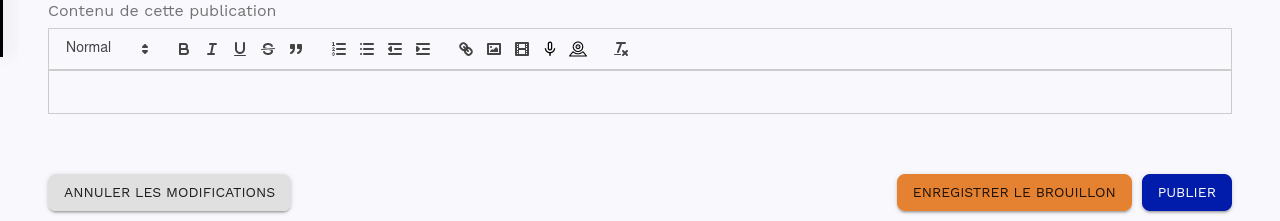
\includegraphics{./Captures/portail.publications.creer.publication.2.classique.png}
	\caption{La seconde partie de la création d'une publication : l'éditeur classique}
\end{figure}
De gauche à droite les icônes permettent :
\begin{itemize}
	\item de structurer le texte sélectionné avec un niveau hiérarchique dans le document,
	\item de mettre la sélection en (on peut cocher plusieurs choix)
		\begin{itemize}
		\item gras
		\item italique
		\item souligné
		\item barré
		\end{itemize}
	\item d'ajouter une citation
	\item d'ajouter une liste numérotée
	\item d'ajouter une liste pucée
	\item de diminuer le retrait du texte sélectionné
	\item d'augmenter le retrait du texte sélectionné
	\item d'ajouter un lien vers une ressource sur internet,
	\item d'insérer une image
	\item d'insérer une vidéo
	\item d'insérer un fichier audio
	\item d'enregistrer et insérer une vidéo (si la webcam existe sur l'ordinateur)
	\item de supprimer les mises en forme de la sélection
\end{itemize}

\paragraph{L'éditeur Markdown}
Markdown est un langage de balisage léger permettant de l'insertion d'objets et du formatage. 
Le chapitre \ref{chap-codimd} se réfère à ce langage tellement pratique qu'il est devenu mon outil de prise de notes pendant les réunions.
\begin{figure}
	\centering
	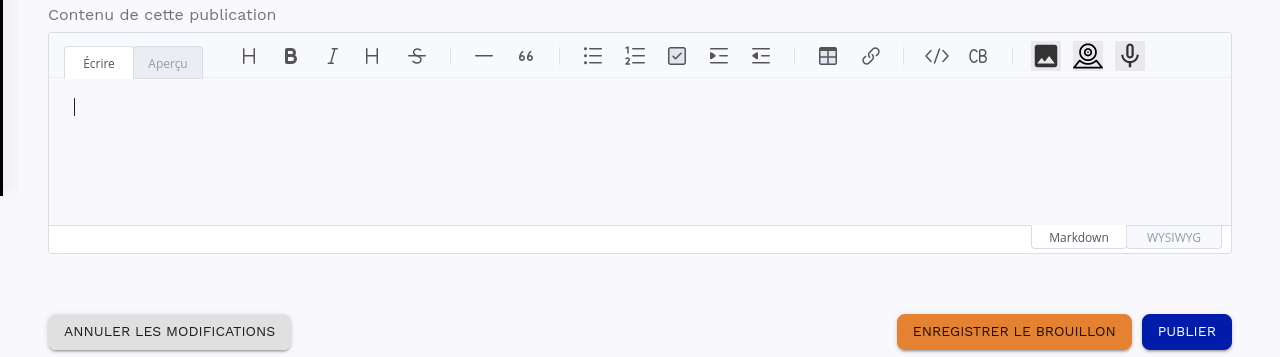
\includegraphics{./Captures/portail.publications.creer.publication.2.markdown.png}
	\caption{}
\end{figure}

\paragraph{Les deux modes acceptés en Markdown.} 
Ce sont le mode Markdown et le mode WYSIWYG\footnote{%
WYSIWYG : \emph{What You See Is What You Get} est un acronyme désignant une famille d'outils numériques, généralement des traitements de textes, où vous avez le formatage et le rendu en même temps que vous le saisissez. 
Cette famille diffère d'autres langages ou logiciels de traitement de texte comme Markdown, Restructured Text ou encore \TeX{} et \LaTeX{} (entre autres) où le formatage est signifié par des balises mais le rendu n'est visible qu'après compilation du document.
}.

L'éditeur Markdown offre la barre suivante avec de gauche à droite~:
\begin{figure}
	\centering
	
\includegraphics{./Captures/portail.publications.creer.publication.barre.markdown.png}
	\caption{L'éditeur Markdown}
\end{figure}
\begin{itemize}
	\item gestion des en-têtes (titre, sous-titre, ...), 
	\item gras,
	\item italique,
	\item choix de la couleur du texte,
	\item texte barré,
	\item ligne horizontale,
	\item citation,
	\item liste pucée,
	\item liste numérotée,
	\item case de tâche à cocher,
	\item augmentation du retrait du texte,
	\item diminution du retrait du texte,
	\item insertion d'un tableau,
	\item insertion d'un lien vers l'extérieur,
	\item insertion d'un code en ligne,
	\item insertion d'un code en bloc,
	\item ajout d'un media (comprendre image),
	\item enregistrement et ajout d'une vidéo,
	\item enregistrement et ajout d'une séquence audio
\end{itemize}

L'éditeur WYSIWYG offre la barre suivante, certaines options de l'éditeur markdown sont soit absentes, soit inactives (grisées clairement)
\begin{figure}
	\centering
	
\includegraphics{./Captures/portail.publications.creer.publication.barre.wysiwyg.png}
	\caption{L'éditeur Markdown-Wysiwyg}
\end{figure}

\paragraph{Enregistrement}
Une fois la note saisie entièrement le bas de la fenêtre offre trois choix, celui de l'annulation, celui de l'enregistrement en tant que brouillon ou bien celui de la publication, comme le montre la capture suivante.
\begin{figure}
	\centering
	
\includegraphics{./Captures/portail.publications.creer.publication.3.png}
	\caption{\emph{this is your last chance}}
\end{figure}

\subsection{Voir toutes les publications}
L'autre bouton important de l'onglet publications ouvre une nouvelle fenêtre, ou un nouvel onglet suivant la configuration de votre navigateur, pour afficher les derniers articles du blog.
\begin{figure}
	\centering
	
\includegraphics{./Captures/portail.publications.afficher.toutes.le.blog.png}
	\caption{Les derniers articles du blog}
\end{figure}

Notez que la barre du haut de la fenêtre est également changée, puisque cette fois-ci c'est celle qui suit qui s'affiche.
\begin{figure}
	\centering
	
\includegraphics{./Captures/portail.publications.afficher.toutes.le.blog.barre.png}
	\caption{La barre du blog}
\end{figure}
Elle permet d'afficher de gauche à droite, l'accueil avec les dernières publications, l'intégralité des publications avec un outil de filtrage par tags, les régions académiques avec les publications rattachées par région ou structure (comme CANOPÉ par exemple), la liste des auteurs et le nombre d'article qu'ils ont publié, la liste des groupes et le nombre de publications associées au groupe, et pour finir les publications lues et marquées comme favorites par vos soins.